\section*{ГЛАВА 2}
\section*{АНАЛИЗ ТРЕБОВАНИЙ К ПРОГРАММНОМУ СРЕДСТВУ}
\addcontentsline{toc}{section}{ГЛАВА 2}
\addcontentsline{toc}{section}{АНАЛИЗ ТРЕБОВАНИЙ К ПРОГРАММНОМУ СРЕДСТВУ}
\label{sec:freq}
\setcounter{section}{2}
\setcounter{subsection}{0}
\bigskip

\subsection{Описание функциональности ПС}
Основываясь на требованиях изложенных в разделе \ref{sec:domain:summary} и диаграмме вариантов использования~(рисунок~\ref{fig:freg:usecase}) разрабатываемое ПС должно выполнять следующие функции:

\begin{itemize}
	\item регистрация пользователя;
	\item авторизация пользователя;
	\item просмотр сохраненных образцов почерка;
	\item добавление нового образца почерка;
	\item выделение признаков образца почерка;
	\item определение психологических характеристик личности;
	\item биометрическая аутентификации пользователя;
	\item определение неврологических отклонений.
\end{itemize}

\begin{figure}[ht]
	\centering
    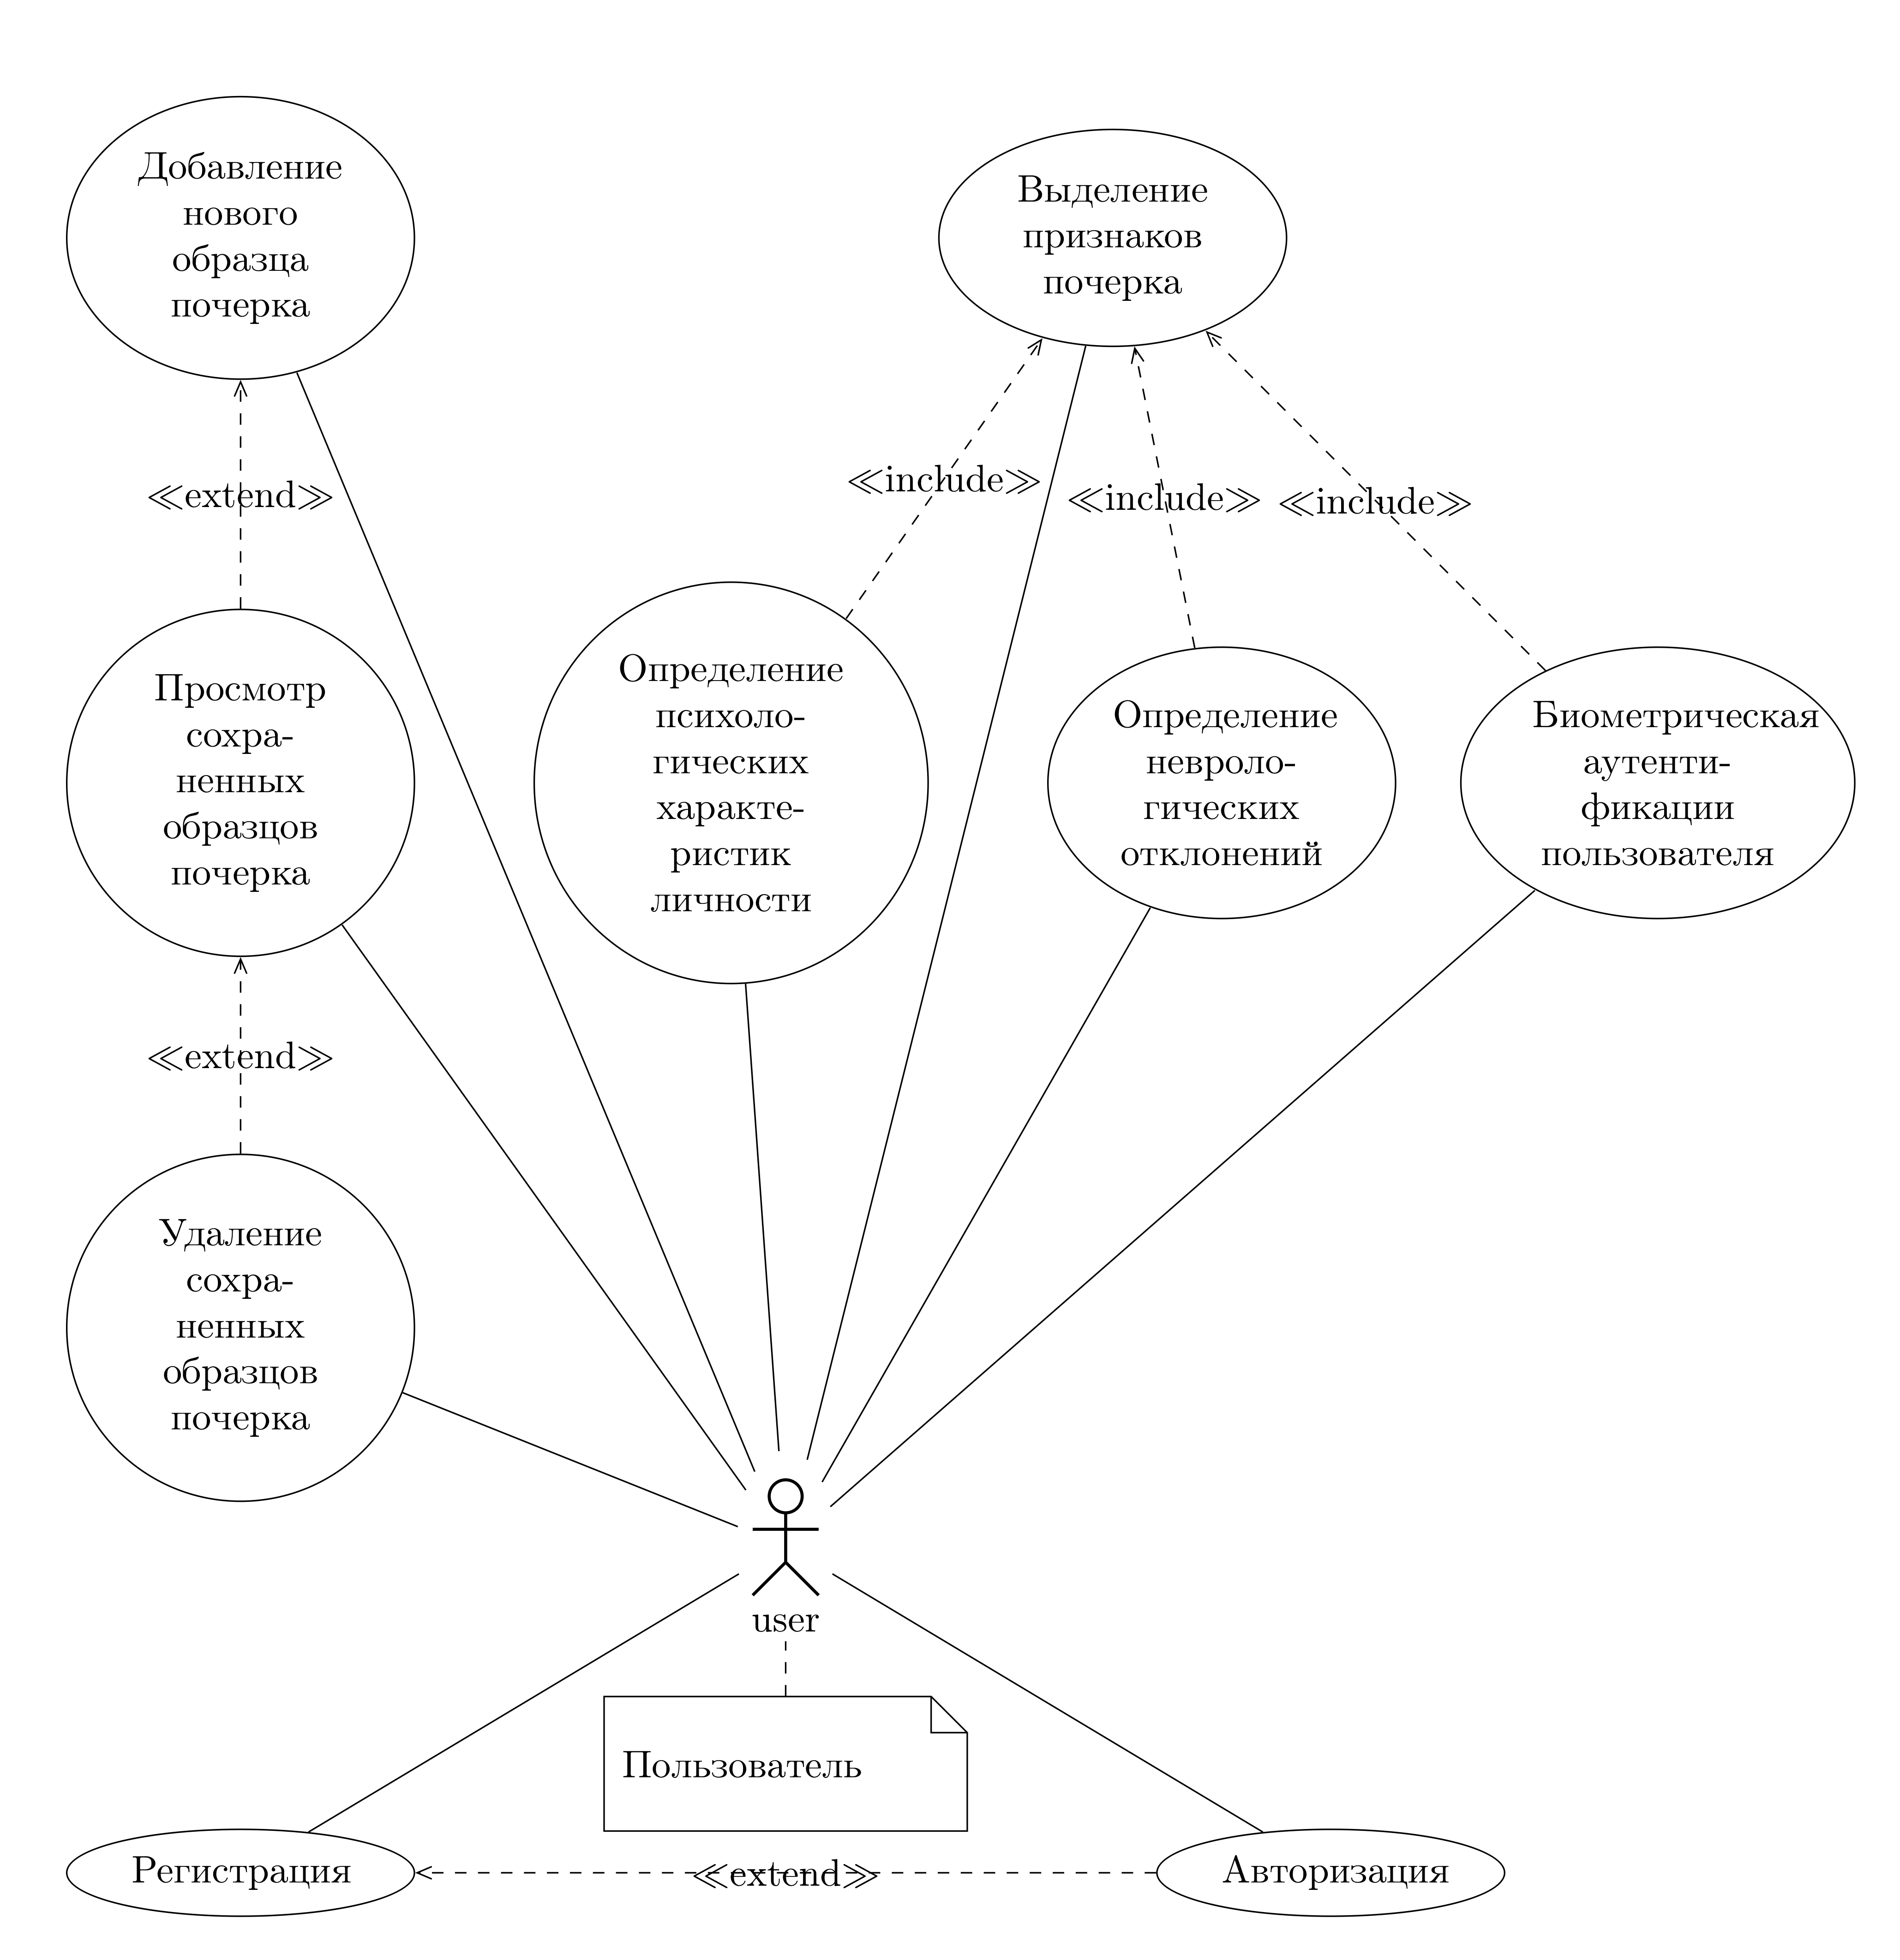
\includegraphics[scale=1.7]{figures/use_case.png}  
    \caption{Диаграмма вариантов использования}
  	\label{fig:freg:usecase}
\end{figure}

Перечисленные функции позволят обеспечить полноценное функционирование программного средства, так как они покрываю все базовые операции хранения данных, а так же включают специализированные операции выделения признаков почерка и из классификации. Так же стоит отметить, что для полноценной промышленного использования программного средства необходимо соблюдение следующих требований:
\begin{itemize}
  \item контроль сложности пароля;
  \item пароль не должен хранится в базе данных в открытов виде;
  \item асинхронное взаимодействие всех компонентов;
  \item параметры текста представляют собой вещественные значения с точностью до четырех знаков после запятой;
  \item использование JWT-маркеры для аутентификации и авторизации пользователей.
\end{itemize}

\subsection{Спецификация функциональных требований}
На основании функций программного средства разработана спецификация требований. 
\subsubsection{Регистрация пользователя}
\label{sec:freq:reg}
\begin{itemize}
	\item возможность регистрации должна быть доступна из пользовательского веб-интерфейса;
	\item пароль при регистрации должен проверяться на сложность(должен содержать не менее восьми символов в верхнем и нижнем регистрах и \mbox{цифры);}
	\item авторизационные данные пользователя должны передаваться по защищенному соединению.
\end{itemize}

\subsubsection{Авторизация пользователя}
\label{sec:freq:auth}
\begin{itemize}
	\item авторизационные данные пользователя должны передаваться по защищенному соединению;
	\item пароль пользователя не должен передаваться в явном виде (вычисления хеша в браузере);
 	\item сообщение об ошибке при вводе неверное логина или пароля не должно сообщать что именно введено неправильно.
\end{itemize}

\subsubsection{Просмотр сохраненных образцов почерка}
\label{sec:freq:show}
\begin{itemize}
	\item список ранее загруженных образцов доступен на главной странице пользователя;
	\item образец и дополнительная информация(признаки почерка, результаты анализа) должны загружаться только после выбора образца из списка;
	\item пользователь имеет возможность запустить процесс анализ образца почерка;
	\item пользователь имеет возможность запустить процесс анализа образца почерка, если процесс выделения признаков почерка еще не был выполнен, то он будет запущен и по окончанию начнется процесс анализа.
\end{itemize}

\subsubsection{Удаление сохраненных образцов почерка}
\label{sec:freq:delete}
\begin{itemize}
	\item возможность удаления сохраненных образцов почерка должна быть доступна из пользовательского веб"=интерфейса страница просмотра образца;
	\item при удалении должно запрашиваться подтверждение действия пользователя с сообщением о последствиях;
	\item реальное удаление образца происходит через неделю после подтверждения удаления пользователем (возможность восстановить файл при ошибочном удалении).
\end{itemize}

\subsubsection{Добавление нового образца почерка}
\label{sec:freq:add}
\begin{itemize}
	\item возможность добавить новый образец доступна на главной странице пользователя;
	\item возможно очистить поле ввода до сохранения образца;
	\item после добавления нового образца пользователь переходит на страницу просмотра образца.
\end{itemize}

\subsubsection{Выделение признаков образца почерка}
\label{sec:freq:extract_features}
\begin{itemize}
	\item возможность выделение признаков образца почерка должна быть доступна из пользовательского веб-интерфейса страница просмотра образца;
	\item выделенные признаки образца почерка передаются по сети в виде JSON-объекта;
	\item выделенные признаки образца почерка хранится в таблице БД;
	\item до завершения выделения признаков на странице отображается индикатор обработки.
\end{itemize}

\subsubsection{Определение психологических характеристик личности}
\label{sec:freq:psiho_analysis}
\begin{itemize}
	\item возможность определение характеристик личности должна быть доступна из пользовательского веб-интерфейса страницы просмотра образца;
	\item характеристики личности передаются по сети в виде JSON-объекта;
	\item характеристики личности хранится в таблице БД;
	\item JSON-объект описывающий характеристики личности содержит текстовое описание и метку класса;
	\item до завершения определения характеристик личности на странице отображается индикатор отработки.
\end{itemize}

\subsubsection{Биометрическая аутентификация пользователя по образцу почерка}
\label{sec:freq:bio_identification}
\begin{itemize}
	\item необходимо добавить как минимум 5 образцов почерка для возможности проведения биометрической аутентификации;
	\item возможность аутентификации должна быть доступна из пользовательского веб-интерфейса главной страницы;
	\item результаты аутентификации передаются по сети в виде JSON-объекта;
	\item JSON-объект описывающий результаты аутентификации содержит текстовое описание и флаг успешности аутентификации;
	\item до завершения аутентификации на странице отображается индикатор отработки.
\end{itemize}

\subsubsection{Определение неврологических отклонений}
\label{sec:freq:neuro_analysis}
\begin{itemize}
	\item возможность определение неврологических отклонений должна быть доступна из пользовательского веб-интерфейса страницы просмотра образца;
	\item результаты анализа передаются по сети в виде JSON-объекта;
	\item JSON-объект описывающий результаты неврологического анализа содержит текстовое описание результатов и вещественное значение вероятности отклонений;
	\item до завершения определение неврологических отклонений на странице отображается индикатор отработки.
\end{itemize}

\subsubsection{Пользовательский интерфейс программного средства}
\begin{itemize}
	\item пользовательский интерфейс представляет собой Web-страницу;
	\item поддержка Google Chrome и Firefox последних версий;
\end{itemize}

Поддержка операционных систем Windows, Linux, MacOS обеспечивается использованием <<тонкого клиента>> и ограничена только поддержкой данными системами версий браузеров.
Разрабатываемое программное средство не должно налагать ограничений на количество обрабатываемых и хранимых образцов почерка.

\subsection{Краткие выводы}
В данном разделе были сформированны и детализированны функции будущему программного средства.
Основными функциями разработываемого ПС должны являтся:
\begin{itemize}
	\item регистрация и авторизация пользователя;
	\item добавление, просмотр и удаление образца почерка;
	\item выделение признаков образца почерка;
	\item определение психологических характеристик личности;
	\item биометрическая аутентификации пользователя;
	\item определение неврологических отклонений.
\end{itemize}

Помимо вышыприведдых функций программное средство должно соблюдение следующих требований для соответсвия современным стандартам разработки программного обеспечения:
\begin{itemize}
  \item контроль сложности пароля;
  \item пароль не должен хранится в базе данных в открытов виде;
  \item асинхронное взаимодействие всех компонентов;
  \item параметры текста представляют собой вещественные значения с точностью до четырех знаков после запятой;
  \item использование JWT-маркеры для аутентификации и авторизации пользователей.
\end{itemize}

Опираясь на вышеизложенную функциональность можно приступать к проектированию архитетесктуры программного средства.